\section{Datasets}
\label{sec:datasets}

In our approach we propose a supervised machine learning algorithm to estimate the page rank using deep graph networks. For this purpose we require labeled data to develop, train, and validate our model.

All dataset versions have OpenPage Rank (Section~\ref{OpenPageRank}) as ground truth. This means that we use the ordered list of domains from OpenPage Rank to enrich them with more information thus to generate our datasets.

The dataset version 1 represents a subset of the dataset version 2. It was created to give us fast and rough estimate on how well CNNs perform on estimating a page rank of a website. The provided data was used to train and evaluate the performance of a CNN on page rank estimation. 

Dataset version 2 was created to enable the evaluation of deep graph networks for page rank estimation. The provided data was used to train and afterwards to evaluate deep graph networks in experiments. 

\subsection{Dataset Version 1}
\label{DatasetVersion1}
The dataset version 1 consists of 100,000 samples in total. We denote a sample from the ground truth as $x$ and from dataset as $X$. A single sample in the ground truth $x$ can be expressed as a tuple consisting of two values:

\begin{center}
	$x  = (r, u)$
	\begin{itemize}
		\item[$r$] The global rank of the domain, according to Open PageRank (Section~\ref{OpenPageRank}), within $[1, 100000]$. 
		\item[$u$] The URL of the domain. For example a string like \texttt{github.com}.
	\end{itemize}
\end{center}

A single sample $X$ in the dataset can be expressed as a tuple consisting of three values:

\begin{center}
	$X = (\tensorsym{I}, r, u)$
	\begin{itemize}
		\item[$\tensorsym{I}$] The screenshot of the domain in image format PNG and in the resolution $1920\times1080$. The screenshot is generated by the datacrawler for the given domain corresponding to the ground truth. For ensuring repeatability, only the upper visible area of the website has been taken into account, which is provided during the initial loading of the website. 
		\item[$r$] The global rank of the domain, according to Open PageRank, within $[1, 100000]$. 
		\item[$u$] The URL of the domain mapped by the Open PageRank list. For example a string like \texttt{github.com}.
	\end{itemize}
\end{center}

\subsection{Dataset Version 2}
\label{DatasetVersion2}

\subsubsection*{The Directed Graph $G$}
\label{TheDirectedGraph}
The directed graph provides a topological view on the given website by representing all associated web pages within the same domain as nodes and connections as arrows. Nodes and arrows of the graph are enriched with local information about the visited web pages. Figure~\ref{fig:PartialDirectedGraph_timodenk.com} exemplary illustrates the partial directed graph for the domain \texttt{timodenk.com} with three webpages represented as nodes with corresponding attributes and edges.

The directed graph $G$ is characterized by a set of nodes $\mathbb{V}$ and edges $\mathbb{A}$. We limit the number of nodes in a graph to eight, since we are not able to express a website in its entirety as a graph and want to keep the dataset in a feasible size. Each node $v \in \mathbb{V}$ represents a web page of the given domain associated with the graph. A node is characterized by the following tuple:

\begin{center}
	$v = (u, \tensorsym{I}, \tensorsym{M},t, l, s, h)$
	\begin{itemize}
		\item[$u$] The exact URL of the web page. Example: \texttt{https://github.com/help}
		\item[$\tensorsym{I}$] The screenshot of web page in image format JPEG and in the resolution $1920\times1080$. 
		\item[$\tensorsym{M}$] The screenshot of web page in image format JPEG and in resolution $375\times 667$, which represents a screenshot taken from a mobile device.
		\item[$t$] The title of web page as can be seen in the tabs bar of a common browser.
		\item[$l$] The time it takes to download all data of web page from the web server in milliseconds.
		\item[$s$] Number of kilobytes downloaded in total for web page (size).
		\item[$h$] Indicator for whether or not the website uses the protocol HTTPS, the value is $\in\left\{\text{true}, \text{false}\right\}$.
	\end{itemize}
\end{center}

Each edge $a$ represents a possible navigation from web page $v_1$ to $v_2$ in the graph $G$. It can be understood as a hyperlink or button found on web page $v_1$ (source), which points to $v_2$ (target) and has the same fully qualified domain name. 

\begin{center}
	$a \in (v_1, v_2, t)$
	\begin{itemize}
		\item[$v_1$] $\in \mathbb{V}$ The source node (web page).
		\item[$v_2$] $\in \mathbb{V}$ The target node that $v_1$ points to.
		\item[$t$] If existent, the text that links from source to target web page.
	\end{itemize}
\end{center}

\begin{figure}
	\centering
	\usetikzlibrary{shapes.multipart}
	\tikzset{
		vertices/.style = {   
			text width=12.0em, align=center,                                           
			draw,
			rectangle split,
			rectangle split parts=7
		}
	}
	\scalebox{.83}{
		\begin{tikzpicture}
		\node[vertices]  (timodenk) at (5,4) {
			\nodepart{one} $u = $ \texttt{timodenk.com}
			\nodepart{two}$ \tensorsym{I} = $ 
\includegraphics[width=.5\textwidth]{resources/timodenk}
			\nodepart{three} $ \tensorsym{M} = $ 
\includegraphics[width=.25\textwidth]{resources/timodenk_mobile}
			\nodepart{four} $ t = $ Timo Denk
			\nodepart{five} $l = 636$ ms
			\nodepart{six} $s = 434$ kb
			\nodepart{seven} $ h = true$
		};
		
		\node[vertices]  (sites) at (10,2) {
			\nodepart{one} $u = $ \texttt{sites.timodenk.com}
			\nodepart{two} $ \tensorsym{I} = $ 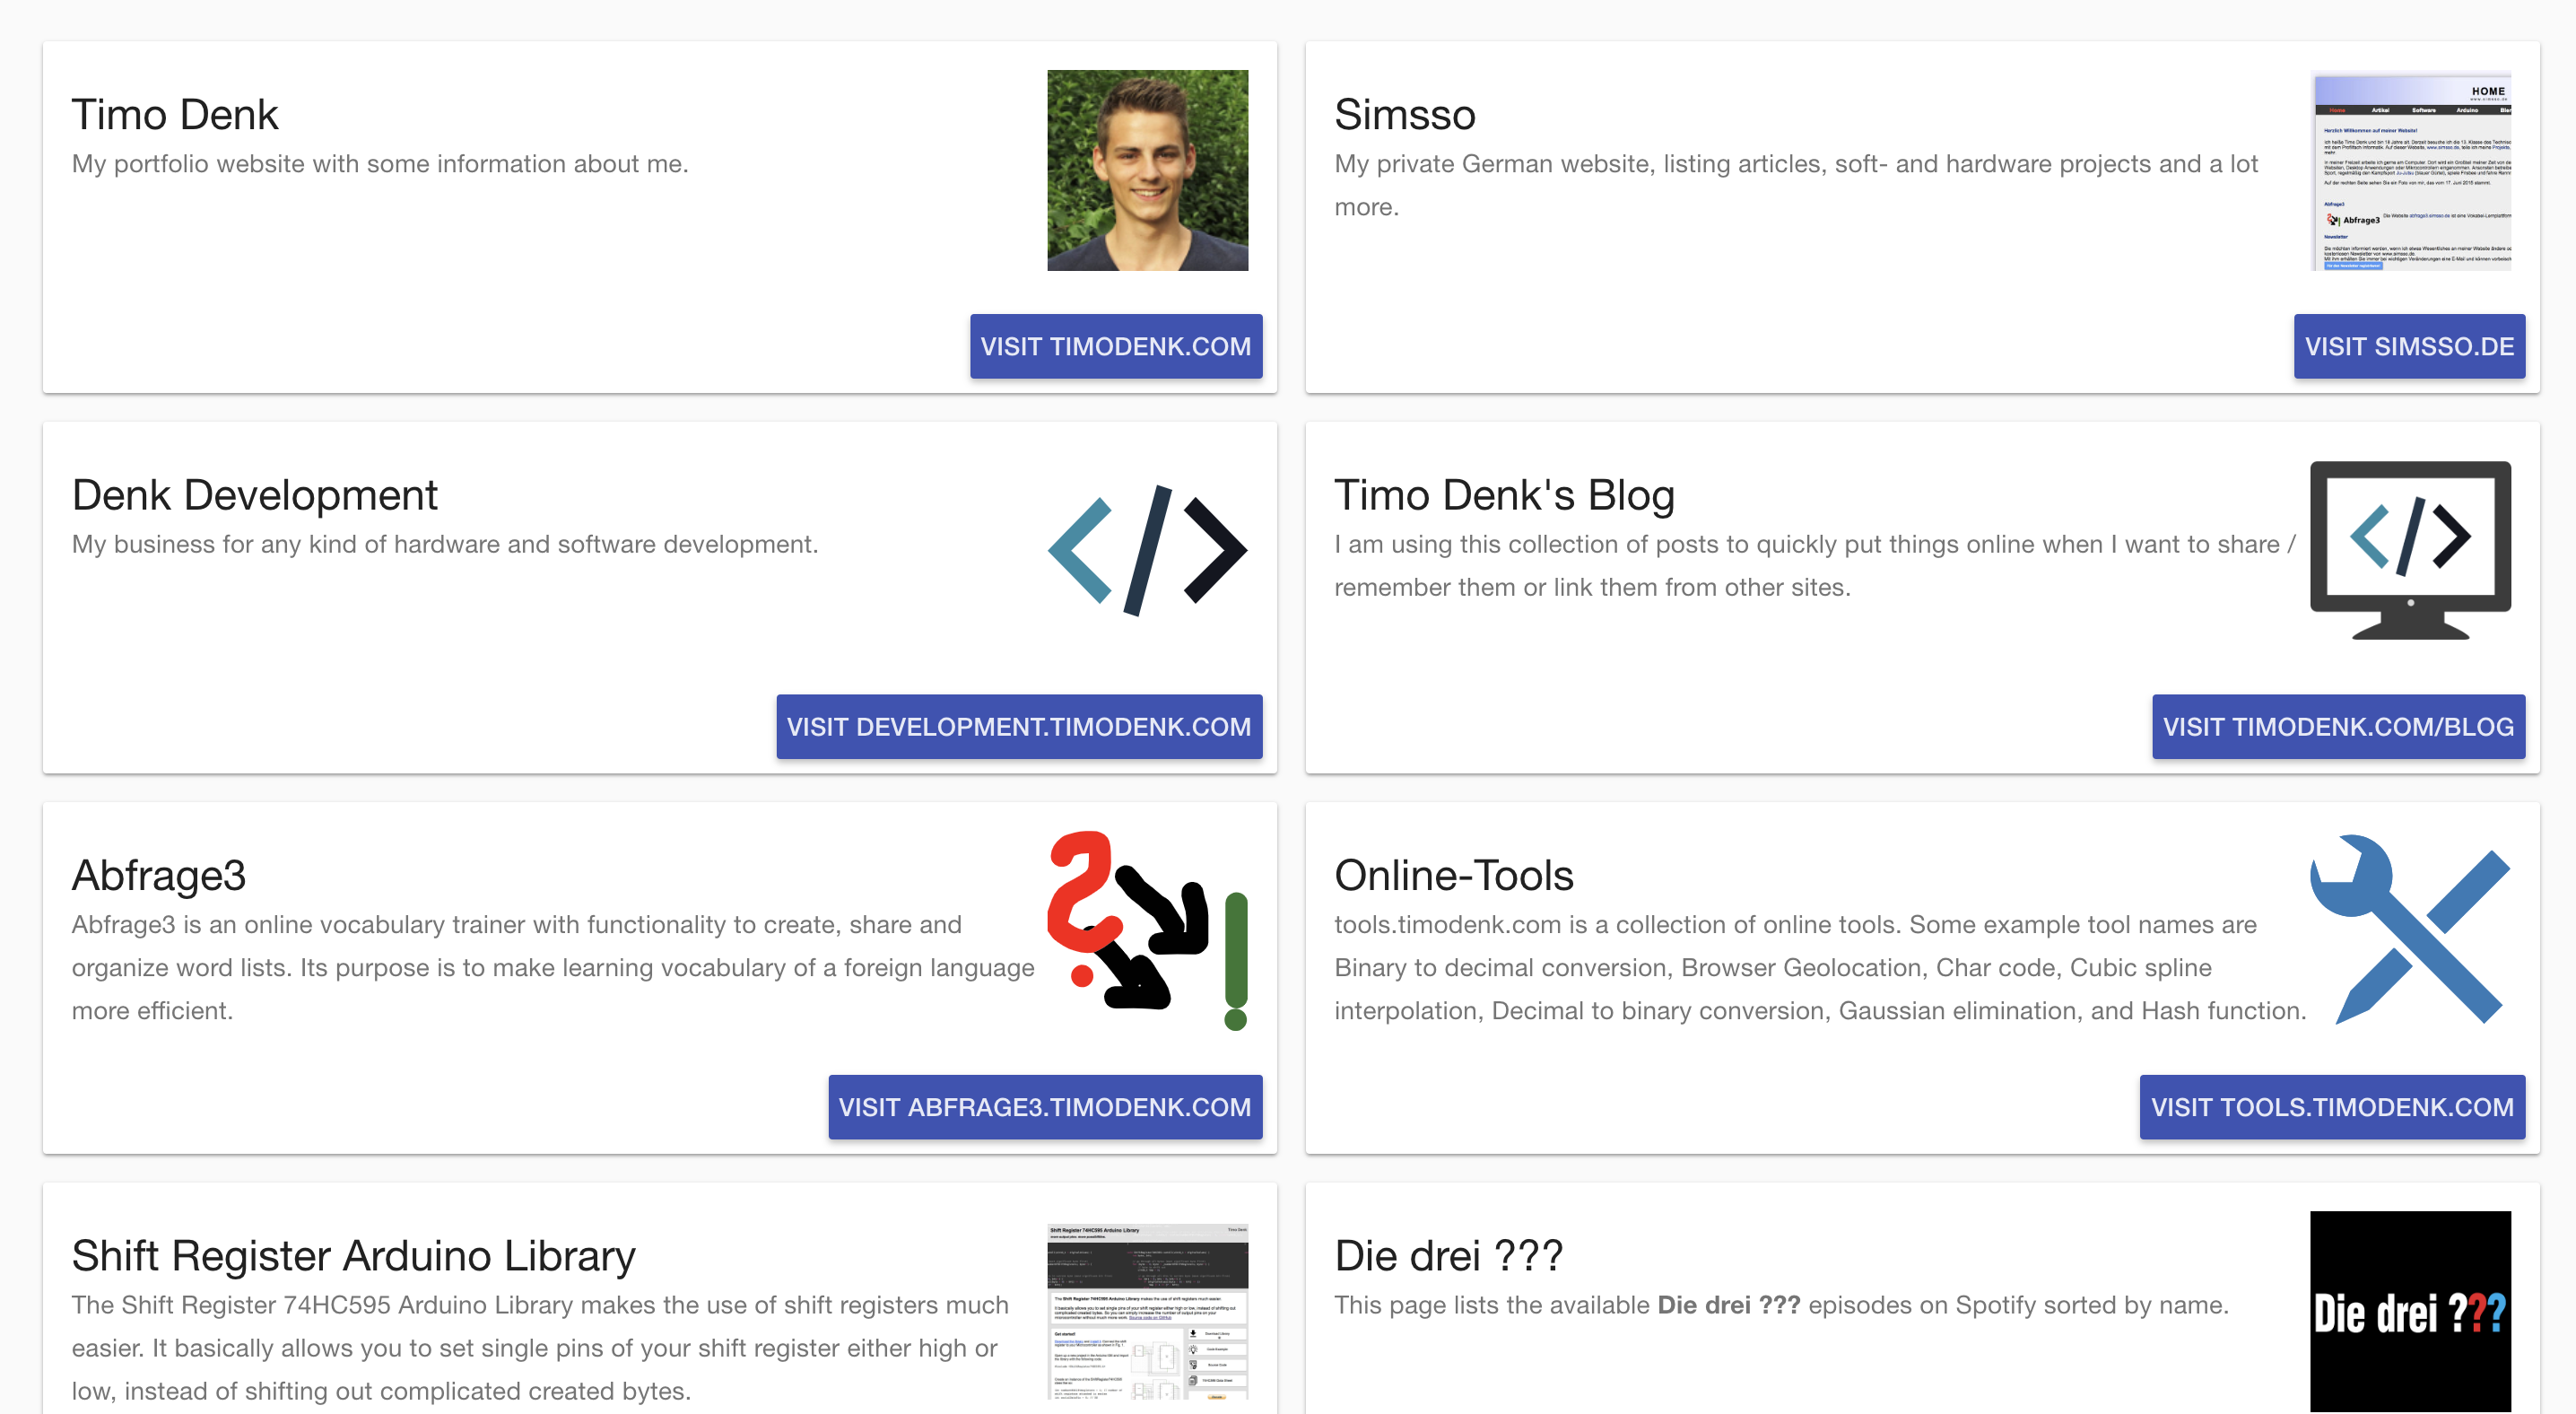
\includegraphics[width=.5\textwidth]{resources/sites_timodenk}
			\nodepart{three} $ \tensorsym{M} = $ 
\includegraphics[width=.25\textwidth]{resources/sites_timodenk_mobile}	\nodepart{four} $ t = $ Timo Denk Sites Overview
			\nodepart{five} $l = 767$ ms
			\nodepart{six} $s = 737$ kb
			\nodepart{seven} $ h = true$
		};
		
		\node[vertices]  (imprint) at (0,2) {
			\nodepart{one} $u = $ \texttt{timodenk.com/imprint}
			\nodepart{two} $ \tensorsym{I} = $ 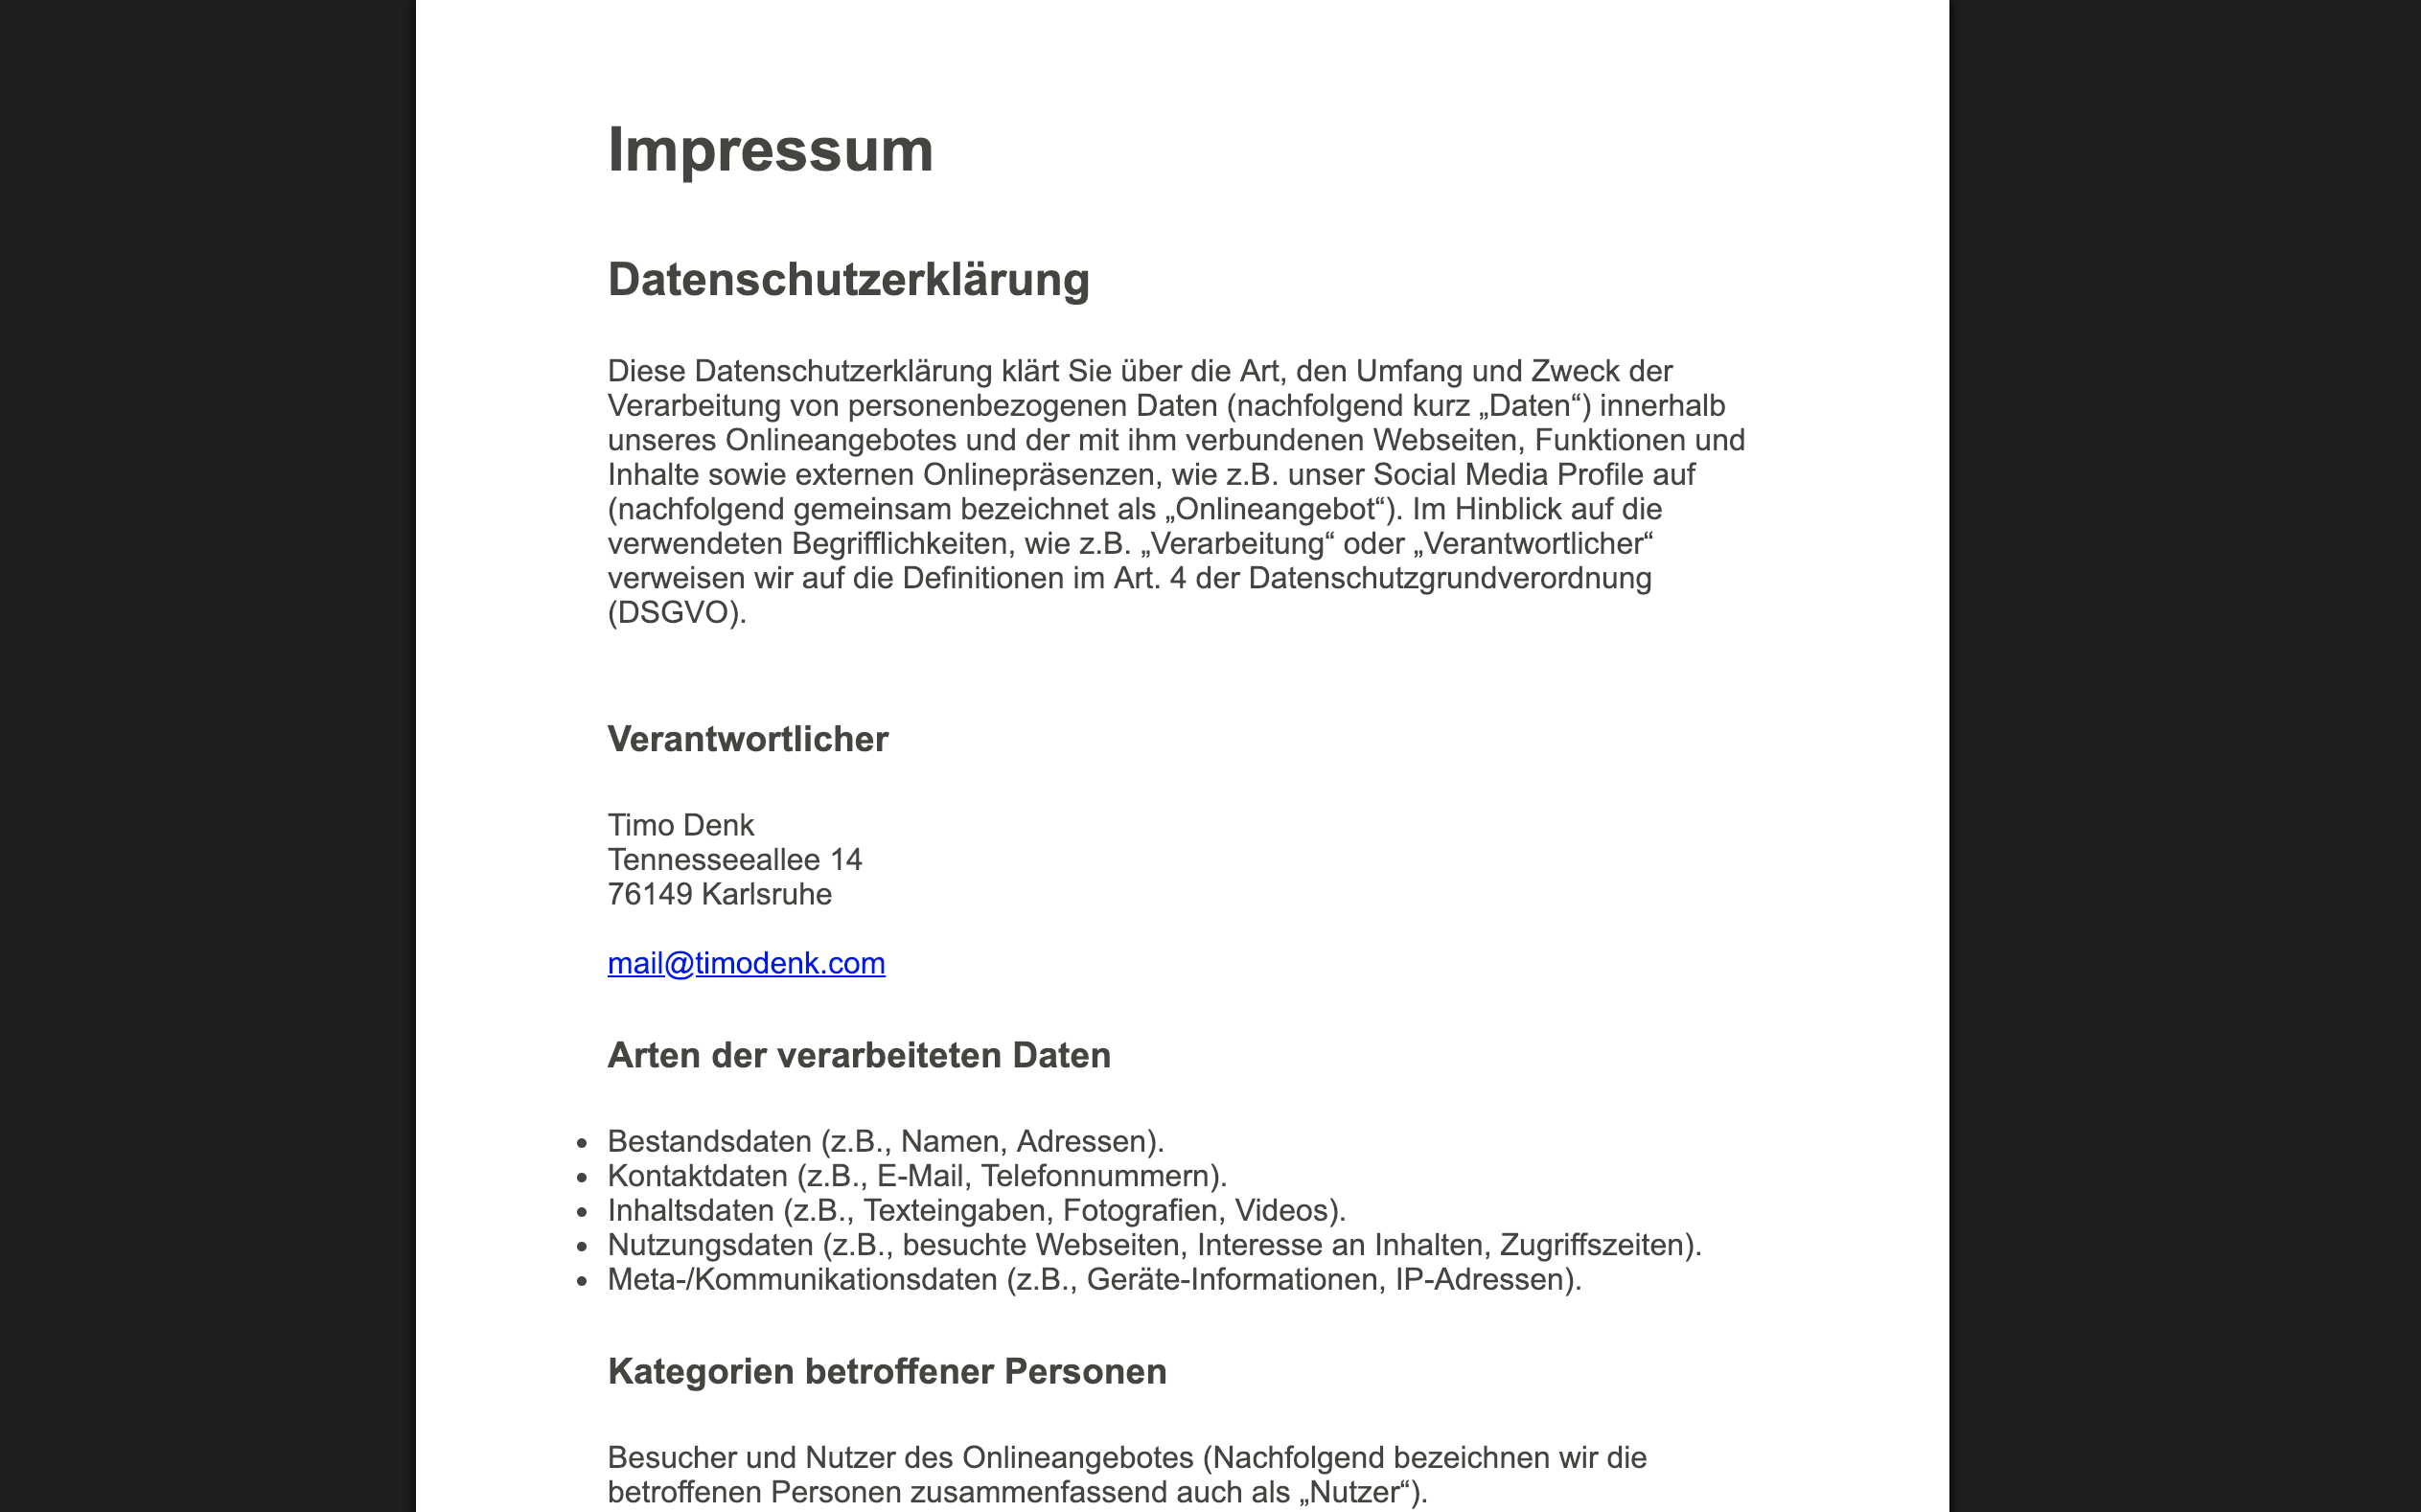
\includegraphics[width=.5\textwidth]{resources/imprint_timodenk}
			\nodepart{three} $ \tensorsym{M} = $ 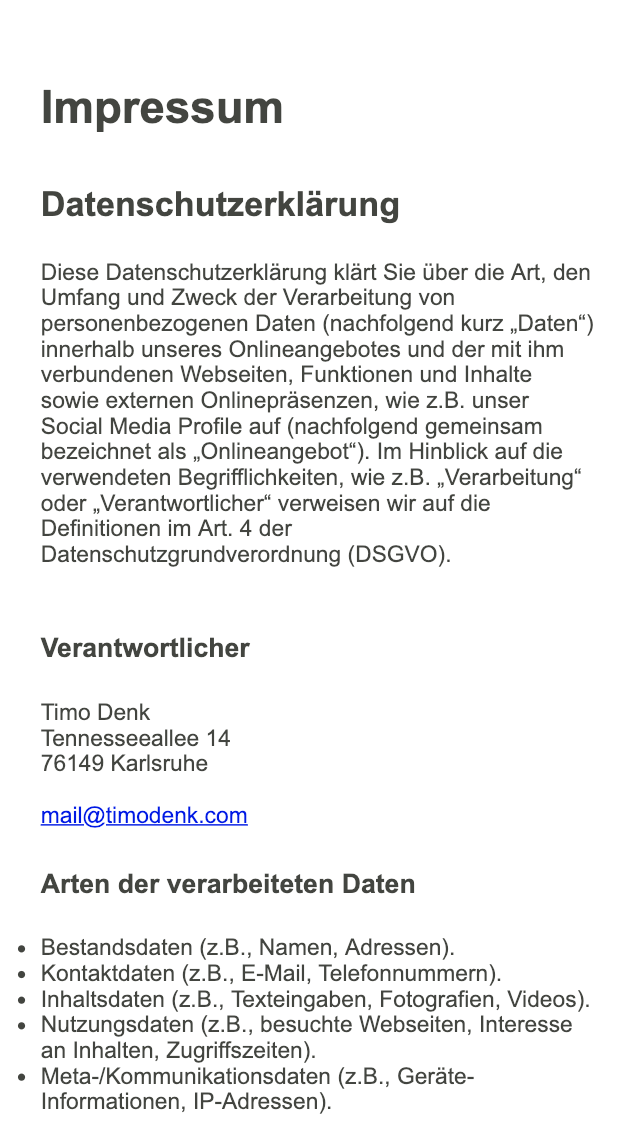
\includegraphics[width=.25\textwidth]{resources/imprint_timodenk_mobile}
			\nodepart{four} $ t = $ Imprint - www.timodenk.com
			\nodepart{five} $l = 304$ ms
			\nodepart{six} $s = 52$ kb
			\nodepart{seven} $ h = true$
		};
		
		\node (timodenkToImprint) at (0.5,6) {$t = $ \texttt{timodenk.com/imprint}};
		\node (timodenkToSites) at (9.5,6) {$t = $\texttt{sites.timodenk.com}};
		\node (SitesToTimodenk) at (5.5,0.25) {$t = $\texttt{timodenk.com}};
		\draw[-latex] (timodenk.one east) to [bend left=30] (sites.one north);
		\draw[-latex] (sites.six west) to [bend left=30] (timodenk.six south);
		\draw[-latex] (timodenk.one west) to [bend right=30](imprint.one north);
		\end{tikzpicture}
	}
	\caption[Example graph as specified by dataset version 2]{The figure illustrates the partial directed graph $G = (\mathbb{V}, \mathbb{A})$ of the domain \texttt{timodenk.com} with three nodes representing the web pages \texttt{timodenk.com}, \texttt{timodenk.com/imprint}, and \texttt{sites.timodenk.com}. Each webpage is a node $v \in \mathbb{V}$ represented as a box containing the tuple of attributes $v = (u, \tensorsym{I}, \tensorsym{M},t, l, s, h)$ as specified in Section \ref{TheDirectedGraph}. Each attribute is represented as an entry in the box and contains respective values of the webpage. For example the webpage \texttt{timodenk.com} contains a screenshot $\tensorsym{I}$ and screenshot in mobile format $\tensorsym{M}$. Furthermore it has the title $t$ "Timo Denk", a loading time $l$ of 636ms, total download size $s$ of 434kb and uses the HTTPS protocol as the value \textit{true} indicates for $h$. Nodes are connected with directed edges $a \in \mathbb{A}$ represented by the arrows in the figure. Moreover, the arrows are annotated exemplary representing the text $t$ that links from the source node $v_1 \in \mathbb{V}$ to the target node $v_2 \in \mathbb{V}$ as specified in Section \ref{TheDirectedGraph}. For example the node of the webpage \texttt{timodenk.com} has an edge $a \in \mathbb{A}$, which points to the node $v_2 \in \mathbb{V}$  of the webpage \texttt{sites.timodenk.com} and has the text $t$ \texttt{sites.timodenk.com}.}
	\label{fig:PartialDirectedGraph_timodenk.com}
\end{figure}

\subsubsection*{Specification}
There are in total 100,000 samples in dataset version 2. Like in dataset version 1, we denote a sample from the ground truth as $x$ and from dataset as $X$ as well. We define a single sample $X$ in the dataset version 2 as a tuple consisting of three values:

\begin{center}
	$X = (G,u,r)$
	\begin{itemize}
		\item[$G$] The directed graph of the domain characterized by a set of nodes $\mathbb{V}$ and edges $\mathbb{E}$: $G= \left(\mathbb{V}, \mathbb{A}\right)$.
		\item[$u$] The URL of the domain mapped by the Open PageRank list.
		\item[$r$] The global rank of the domain, according to Open PageRank, within $[1, 100000]$. 
	\end{itemize}
\end{center}